\documentclass{cmspaper}
\usepackage{graphicx}
\usepackage{rotate}
\usepackage{relsize}
\newcommand{\met} {\ensuremath{E\!\!\!\!/_T}}
\newcommand{\ttbar} {\ensuremath{t\bar{t}~}}
\newcommand{\ptll} {\ensuremath{P_T(\ell\ell)}}
\newcommand{\ptllres} {\ensuremath{P^{\rm res}_T(\ell\ell)}}

\begin{document}

%==============================================================================
% title page for many authors
%
\begin{titlepage}
\title{SUSY sensitivity and discovery potential using di-leptons at $\sqrt{s} = 7 $ TeV}

  \begin{Authlist}
    D.~ Barge, C.~Campagnari, P.~Kalavase, D.~Kovalskyi, V.~Krutelyov, J.~Ribnik
    \Instfoot{ucsb}{University of California, Santa Barbara}
    W.~Andrews, D.~Evans, F.~Golf, J.~M\"ulmenst\"adt, S.~Padhi, Y.~Tu, F.~W\"urthwein, A.~Yagil
    \Instfoot{ucsd}{University of California, San Diego}
    L.~Bauerdick, I.~Bloch, K.~Burkett, I.~Fisk, Y.~Gao, O.~Gutsche, B.~Hooberman
    \Instfoot{fnal}{Fermi National Accelerator Laboratory, Batavia, Illinois}
  \end{Authlist}

\begin{abstract}
SUSY sensitivity and discovery potential using di-leptons at $\sqrt{s} = 7 $ TeV
are presented in this note. The mass reach as well as CMS sensitivity to several regions in
parameter space are evaluated within the framework of minimal supergravity and assuming R-parity
conservation. These studies are performed for inclusive searches involving same and opposite 
sign di-leptons. The new physics is characterized by large \met~ and significant hadronic 
activity. The study shows significant sensitivity in several regions in the parameter 
space with 100 pb$^{-1}$ and 1 fb$^{-1}$ of integrated luminosity.
\end{abstract}
\end{titlepage}

\section{Introduction}
\label{sec:intro}

After the successful operation of the Large Hadron Collider (LHC) and the CMS detector
in 2010 and 2011, and with good prospects for the future, the LHC is now ready to shed light on a number 
of open questions in Particle Physics 
such as the mechanism of electroweak (EW) symmetry breaking, or the 
new physics, Beyond the Standard Model (BSM), that stabilizes the EW scale. 

A wealth of theories that extend the Standard Model have been put forth during the past decades. Supersymmetry (SUSY) is
arguably the best motivated BSM theory --- and certainly the most 
thoroughly studied. 
Indeed, searches for SUSY are among the primary objectives of the 
CMS experiment. SUSY is exceedingly popular not 
only for its theoretical beauty but also because SUSY phenomenology 
is extremely rich, 
%in fact is can mimic almost any other new physics scenario. 
leading to a large variety of possible new signals at the LHC. 
In spite of this, the majority of SUSY studies focus on a very special 
setup: the so-called Constrained Minimal Supersymmetric Standard Model (CMSSM). 
This was justified in the preparation for discoveries as the CMSSM, 
having just a handful of new parameters, is very predicive. However, 
the simplifying assumption of universality at the GUT scale lacks a sound 
theoretical motivation. Consequently, the CMSSM should be regarded as a showcase 
model. When it comes to interpreting experimental results, it is reasonable and interesting to do this within the CMSSM because it 
provides (to some degree) an easy way to show performances, 
compare limits or reaches, etc. However, the interpretation of experimental results in the 
$(m_0,m_{1/2})$ plane risks imposing unwarranted constraints on SUSY, as many 
mass patterns and signatures that are possible a priori are not covered in the CMSSM. 
The same problem arises in any analysis that assumes a particular 
SUSY breaking scheme. 

In this document, we therefore introduce a different approach, which uses only 
minimal assumptions on the underlying SUSY parameters. In particular, given the absence of experimental guidance, we choose
not to rely on a particular SUSY breaking scheme.
Instead, we use a 19-dimensional 
parametrization of the MSSM, called the \emph{phenomenological MSSM} (pMSSM),
with parameters defined not at the GUT scale but instead at the SUSY scale 
(by convention the geometric mean of the two stop masses).
We demonstrate the feasibility of our approach by applying it to 
the 2011 CMS data-set corresponding to 1~fb$^{-1}$ of integrated luminosity.  
Using profile likelihoods, we combine 
the dijet $\alpha_T$ analysis, the opposite-sign dilepton 
analysis and the same-sign dilepton analysis and derive constraints 
on the SUSY particles with as few simplifying assumptions as possible.
Results from other SUSY analyses in CMS will be added as soon as they become available.

We first give the motivation to go beyond the CMSSM and work in 
a generic MSSM setup. After this, the pMSSM and its parametrization is defined. 
We then outline our analysis, giving details on the pMSSM points we have used, 
the detector simulation and the CMS analyses, and describe the statistical method based on 
profile likelihoods used for coping with the 19-dimensional model. Finally, we discuss our results and summarize our conclusions.


\section{Data Samples}
\label{sec:datasamples}
This study is based on the 2\_2\_X re-reco full simulation data samples
listed in Table~\ref{tab:datasets}.  The Standard Model (SM) data sets have been normalized 
to the cross-sections compiled by the top group~\cite{tosi};  for the SUSY 
data sets we used the cross-sections from the Summer 2008 production 
page~\cite{summer08}.

\begin{table}[hbt]
\begin{center}
\begin{tabular}{|l|}\hline
{\tt /TTJets-madgraph/Fall08\_IDEAL\_V11\_redigi\_v10/GEN-SIM-RECO} \\
{\tt /WJets-madgraph/Summer08\_IDEAL\_V11\_redigi\_v1/GEN-SIM-RECO} \\
{\tt /ZJets-madgraph/Summer08\_IDEAL\_V11\_redigi\_v1/GEN-SIM-RECO} \\
{\tt /WW/Summer08\_IDEAL\_V11\_redigi\_v1/GEN-SIM-RECO} \\
{\tt /WZ\_incl/Summer08\_IDEAL\_V11\_redigi\_v1/GEN-SIM-RECO} \\
{\tt /ZZ/Summer08\_IDEAL\_V11\_redigi\_v1/GEN-SIM-RECO} \\
{\tt /SingleTop\_sChannel/Summer08\_IDEAL\_V11\_redigi\_v3/GEN-SIM-RECO} \\
{\tt /SingleTop\_tWChannel/Summer08\_IDEAL\_V11\_redigi\_v3/GEN-SIM-RECO} \\
{\tt /SingleTop\_tChannel/Summer08\_IDEAL\_V11\_redigi\_v3/GEN-SIM-RECO} \\
{\tt /SUSY\_LM0-sftsht/Summer08\_IDEAL\_V11\_v1/GEN-SIM-RECO} \\
{\tt /SUSY\_LM*-sftsht/Summer08\_IDEAL\_V11\_redigi\_v1/GEN-SIM-RECO} \\
\hline
\end{tabular}
\caption{The data sets used in this study.\label{tab:datasets}}
\end{center}
\end{table}

Monte Carlo events were analyzed with CMSSW\_2\_2\_10 
with the additional tags listed in Table~\ref{tab:tags}.

\begin{table} [htb]
\begin{center} 
\begin{tabular}{|l|} \hline
{V01-08-04 CondFormats/JetMETObjects} \\
{V00-06-02-09 DataFormats/METReco} \\
{V07-02-12-03 DataFormats/MuonReco} \\
{V01-08-02-01 JetMETCorrections/Algorithms} \\
{V01-08-15 JetMETCorrections/Configuration} \\
{V03-02-06 JetMETCorrections/JetPlusTrack} \\
{V02-09-02 JetMETCorrections/Modules} \\
{VB04-00-02-04 JetMETCorrections/Type1MET} \\
{V01-04-03 RecoJets/JetAssociationAlgorithms} \\
{V00-04-02-17 RecoMET/Configuration} \\
{V02-05-00-21 RecoMET/METAlgorithms} \\
{V02-08-02-17 RecoMET/METProducers} \\
{V03-26-04 DataFormats/PatCandidate} \\
{V05-05-09 PhysicsTools/PatAlgos} \\
{V03-06-03 PhysicsTools/PatUtils} \\
{V03-01-16 PhysicsTools/PFCandProducer} \\
{V09-30-03 PhysicsTools/HepMCCandAlgos} \\
{V05-13-02 DataFormats/HepMCCandidate} \\
\hline
\end{tabular}
\caption{Additional software tags used in this study.\label{tab:tags}}
\end{center}
\end{table}

\section{Event Selection}
\label{sec:eventselection}

The event selection used is not optimized for any specific non-standard model 
scenario. It is based on small modifications to the baseline 
di-lepton event selection that we used in our same-sign published study~\cite{ssnote1, sspaper}. The 
only difference is that we now require both leptons to have the transverse 
momentum ($p_t$) $> 20$ GeV. A quick summary of the event selection is:

\begin{itemize}
\item We require a mixture of unprescaled single and double lepton triggers as mentioned in~\cite{ssnote1}.
 The combined trigger efficiency is $\sim 99.9 \pm 0.1$\% for di-lepton events that pass the event selection.
\item At least two isolated same sign leptons ($ee$, $e\mu$, and $\mu\mu$). 
\item Leptons must have $P_T > 20$ GeV, $|\eta|< 2.4$.
\item We consider L2L3 corrected particle flow Jets with $P_T > 30$ GeV and
	$|\eta|< 2.4$.
\item The scalar sum of the $P_T$ of all jets passing the requirements above should be $>$ 60 GeV.
\item At least two jets.
\item We remove di-lepton events with invariant mass $ < 5$ GeV.

\item Additional Z-Veto:
\begin{itemize}
      \item  we veto the candidate lepton, if an extra lepton in the event pairs with the candidate lepton
             to form a $Z$ within the mass range between $76 < m_{\ell\ell} $ (GeV) $< 106$. This requirement is 
             designed to reject $WZ$ events.
\end{itemize}
\item We require particle flow \met~$>$ 30(20) GeV for $ee,\mu\mu (e\mu)$ events. 
We find that both tcMET and pfMET lead to similar results.
\item We require that all three charge measurements from GSF, CTF and Supercluster Charge algorithms agree. The
Supercluster Charge is determined from the relative position of the supercluster with respect to the projected
track from the pixel seed.
\end{itemize}
\noindent More details on the selections can be found elsewhere~\cite{ssnote1, sspaper}.

%\section{Statistical Methods}
\label{sec:mSUGRA}



\section{Search for Same Sign Top Quark Pair Production}
\label{sec:samesign}

This analysis is based on the approved same-sign di-lepton search documented in AN 2010/247 v6 \cite{ssnote1}
and corresponds to an integrated luminosity of 35 pb$^{-1}$.
In that analysis we searched for events with two isolated same sign leptons, two or more jets, and MET ($\met$).
This final state is exactly the final state that one would expect from top-top production with 
both top quarks decaying as $t\rightarrow Wb$, $W\rightarrow \ell \nu$.



\subsection{Event Selection}

In AN 2010/247 we presented event yields and background expectations for several event selections.  
One of those event selections is very similar to that of the $t\bar{t}$ (opposite sign) dilepton 
cross-section analysis \cite{topxsection}, 
and thus it is the appropriate selection for a top-top pair search.  
Briefly, this selection consists of

\begin{itemize}
	\item Two same sign leptons of $p_T>20$ GeV, $|\eta|<2.4$
	\item Two jets of $p_T>30$ GeV, $|\eta|<2.4$
	\item $\met >20$ GeV ($e\mu$) or $\met>30$ GeV ($ee$ or $\mu\mu$)
\end{itemize}

\noindent More details are to be found in Reference~\cite{ssnote1}.

\subsection{Event Yields and Background}
\label{sec:ssyields}

The results of the search in this kinematical region are 
summarized in Table 6 of AN 2010/247 v6 \cite{ssnote1}, 
which is reproduced below as Table \ref{tab:ssyields}.

The data-driven background prediction is based on a combination 
of estimating ``fake leptons''~\cite{fakenote} (FakeRate) 
and electrons reconstructed with the wrong sign~\cite{ssnote1} (Charge FlipRate). 
The probability for muons to be reconstructed with the wrong sign at the 
relevant momenta is negligible.





%%% Commented out DLE
%This section summarizes the results of the search for same sign $tt$
%pair production in the di-lepton channel. We use two data-driven methods 
%to estimate background characterized by the presence of two isolated high $P_T$ same 
%sign leptons, $\met$, and significant hadronic activity. For the purpose of this note we 
%restrict ourselves to the $ee$, $e\mu$, and $\mu\mu$ final states, {\em i.e.}, we do not 
%consider $\tau$'s, except in the case that the $\tau$ decays leptonically. 
%%%
%As we will show in Section~\ref{sec:ssyields}, for this modified baseline selection is similar to
%the published opposite sign di-lepton pair production cross section paper~\cite{topxsection}, where the main 
%background is from SM \ttbar decays. The data-driven background prediction is based on a combination 
%of estimating ``fake leptons''~\cite{fakenote} (FakeRate) and electrons reconstructed with the 
%wrong sign~\cite{ssnote1} (Charge FlipRate). The probability for muons to be reconstructed with 
%the wrong sign at the relevant momenta is negligible.





%after applying the event selections
%described in Section~\ref{sec:eventselection} to the datasets described in Section~\ref{sec:datasamples} 
%are detailed below. The final event yields also include the systematic uncertanities of
%the method used.

\vspace{6 mm}
\begin{table}[htb]
\begin{center}
\begin{tabular}{|c|c|c|c|c|}
\hline
Sample & $e^{\pm}e^{\pm}$    & $\mu^{\pm}\mu^{\pm}$ & $e^{\pm}\mu^{\pm}$      & total \\ \hline
% all the MCs
\hline
DY  & 0.00000 $\pm$ 0.00000 & 0.00000 $\pm$ 0.00000 & 0.00000 $\pm$ 0.00000 & 0.00000 $\pm$ 0.00000 \\ 
t$\overline{t}$  & 0.03700 $\pm$ 0.01170 & 0.04440 $\pm$ 0.01282 & 0.09250 $\pm$ 0.01850 & 0.17391 $\pm$ 0.02537 \\ 
wjets  & 0.10860 $\pm$ 0.10860 & 0.00000 $\pm$ 0.10860 & 0.00000 $\pm$ 0.10860 & 0.10860 $\pm$ 0.18810 \\ 
tw  & 0.00079 $\pm$ 0.00079 & 0.00079 $\pm$ 0.00079 & 0.00475 $\pm$ 0.00194 & 0.00634 $\pm$ 0.00224 \\ 
single top t-ch.  & 0.00138 $\pm$ 0.00138 & 0.00000 $\pm$ 0.00138 & 0.00276 $\pm$ 0.00195 & 0.00415 $\pm$ 0.00276 \\ 
single top s-ch.  & 0.00000 $\pm$ 0.00012 & 0.00035 $\pm$ 0.00020 & 0.00023 $\pm$ 0.00016 & 0.00058 $\pm$ 0.00028\\ 
ww  & 0.00000 $\pm$ 0.01219 & 0.00000 $\pm$ 0.01219 & 0.01219 $\pm$ 0.01219 & 0.01219 $\pm$ 0.0211 \\ 
wz  & 0.01109 $\pm$ 0.00784 & 0.01109 $\pm$ 0.00784 & 0.07207 $\pm$ 0.01999 & 0.09425 $\pm$ 0.02286 \\ 
zz  & 0.00000 $\pm$ 0.00178 & 0.00178 $\pm$ 0.00178 & 0.00535 $\pm$ 0.00309 & 0.00713 $\pm$ 0.00356 \\ 
\hline
Total MC  & 0.15886 $\pm$ 0.10952 & 0.05841 $\pm$ 0.01515 & 0.18986 $\pm$ 0.03012 & 0.40713 $\pm$ 0.11459 \\
\hline\hline
data  (35 pb$^{-1}$)     & 0  &  0  & 2  & 2      \\ \hline
fake rate prediction & & & & \\ \hline
single fake   & 0.47105 $\pm$ 0.33308 & 0.12058 $\pm$ 0.12058 & 1.05798 $\pm$ 0.48320 & 1.64961 $\pm$ 0.59914 (8 evts) \\
double fake   & 0.00000 $\pm$ 0.24180 & 0.00000 $\pm$ 0.02086 & 0.00000 $\pm$ 0.07102 & 0.00000 $\pm$ 0.25288 (0 evts) \\
fake prediction & 0.47105 $\pm$ 0.41159 & 0.12058 $\pm$ 0.12237 & 1.05798 $\pm$ 0.48839 & 1.64961 $\pm$ 0.65032 \\
\hline
flip rate prediction & $0.06\pm 0.01$ & 0 & $0.02\pm 0.003$ & $0.08\pm 0.01$ \\ \hline\hline
total data driven prediction & $0.54\pm 0.48$ & $0.13\pm 0.14$ & $1.07\pm 0.72$ & $1.74\pm 1.05$ \\ \hline
total MC driven prediction & $0.01\pm 0.01$ & $0.01\pm 0.01$ & $0.08\pm 0.04$ & $0.10\pm 0.05$ \\\hline\hline
total bkg prediction & $0.55\pm 0.48$ & $0.14\pm 0.14$ & $1.15\pm 0.7$ & $1.8\pm 1.1$ \\\hline
\end{tabular}
\caption{\protect Data and Monte Carlo yields for the same sign di-leptons with $P_T >20$\ GeV
from Reference~\cite{ssnote1}.  Note that this Table inludes $\ell^+\ell^+$ as well
as $\ell^-\ell^-$; Both signal events are $e^+\mu^+$.
Uncertainties in the lower three rows also include the systematic 
uncertanities on the method used.\label{tab:ssyields} }
\end{center}
\end{table}

The event yields have the following characteristics:

\begin{itemize}
\item We do not consider rare processes such as $qqW^\pm W^\pm, WWW, t\bar{t}W$, double parton $W^\pm W^\pm$, which are 
negligibly small~\cite{ssnote1}.
% \item We found small contributions (0.01 events) from conversion of prompt photons in $W/Z\gamma$ using MC and are
% not considered in order to avoid double counting in the single fake contributions.
\item The diboson backgrounds $WW, WZ, ZZ$ are taken from the MC as an additional background estimate. This contribution
is tabulated as the total MC driven predicition.
\item The prediction from fake rates includes the systematic error of 50\%. 
\item The flip rate prediction also includes an additional systematic error of 50\% based on statistics of the same
sign events observed in the control region~\cite{ssnote1}.
\item The systematic errors are added when propagating the fake/flip rates into total data-driven predictions.
\item All MC driven predictions also assume a flat 50\% systematic error.
\end{itemize}

The dominant SM contribution is from \ttbar decays. The total estimated background 
is obtained after the application of Fake and Charge Flip rates 
to the dilepton dataset\cite{ssnote1}. 
The data yield is in good agreement with the background prediction. 
% from both MC as 
% well as the data driven predictions. 

We take the results of Table \ref{tab:ssyields} with one important modification: 
since we are interested in $tt$ production and not $\bar{t}\bar{t}$ production,
we only consider $\ell^{+}\ell^{+}$ events.  
Thus the BG estimates in Table \ref{tab:ssyields} have to be divided by two.
Strictly speaking the W$+$jets background, which according to MC is about 25\%
of the total, is not completely charge symmetric.  
This BG is calculated in a data 
driven was using the fake rate method.  We have repeated the fake rate calculation
of Table~\ref{tab:ssyields} for positive leptons only; the result is 
0.6 events, which is consistent with being one half of the estimate for both
positive and negative leptons of Table~\ref{tab:ssyields} (1.65 events divided
by 2 = 0.8). 

Both observed events in Table \ref{tab:ssyields} have positive leptons.  
Then, the bottom line yield and bg prediction is: 
two events observed and $0.9 \pm 0.6$ expected BG, 
which corresponds to one half the background of Table \ref{tab:sm_preditcion}.
Thus, we see no statistically significant evidence for $pp \to tt$.




% One of the key components of same-sign top pair search is the fact that the final state includes  
% includes mainly one type of sign. 
% For example, in the t-channel exchange: $ uu \rightarrow tt \rightarrow l^+ l^+ \mu \nu b b$ only positively charged leptons are involved. 
% The quark quark, $\bar{u}\bar{u}$ scattering is highly suppressed due to the parton luminosities, thus we do not expect any significant contribution 
% from negatively charged leptons. 
% Given that the data driven methods are robust against any given choice of lepton charge~\cite{fakenote1}, we use half of the total background prediction for this search.


% The results is summarized in Table~\ref{tab:sm_preditcion}.

\begin{table}[hbt]
\begin{center}
\begin{tabular}{|l|c|}\hline
Same sign di-leptons & Event yield \\ \hline
Total Observed & 2 \\
Total Predicted & 0.9 $\pm$ 0.55 \\
\hline
\end{tabular}
\caption{ Observed and predicted number of events passing the event selection in 35 pb$^{-1}$ of integrated luminosity. 
The uncertainty also includes systematic errors.\label{tab:sm_preditcion}}
\end{center}
\end{table}

%The ``anatomy'' of the 2 observed event is discussed in the appendix.
% Although the observed events have two positively charged 
% di-leptons, we do not consider this a significant deviation from the prediction.

\subsection{Systematic Uncertainties on the Acceptance}
\label{sec:sssystematics}

The methods used to determine the systematic uncertaintare are discussed in Reference~\cite{ssnote1}.
For lepton selections, we take the result from ~\cite{ssnote1}.
We have recalculated the systematic uncertainties due to ISR/FSR, PDFs, and jet energy scale
appropriate to the $pp \to tt$ process.  The results are 
summarized 
in Table \ref{tab:systSumm}.

\begin{table}[h]
\begin{center}
\begin{tabular}{lcccc}\hline
Source 					& $ee$		& $\mu\mu$		& $e\mu$			& all \\ \hline
Lepton selection			& 11.8\%		& 10.6\%		& 10.8\%			& 10.7\% \\
Energy scale				& 8\%		& 8\%		& 8\%			& 8\% \\
ISR/FSR and PDF				& 3\%		& 3\%		& 3\%			& 3\% 	\\
Total without luminosity		& 14.6\%		& 13.6\%		& 13.8	& 13.7\%	\\ \hline
Integrated luminosity			& 4\%		& 4\%		& 4\%			& 4\%	\\ \hline
Total & 15\% & 14\% & 14\%  & 14\% \\
%%% Total & 13.6\% & 12.4\% & 12.5\%  & 12.5\% \\
\hline
\end{tabular}
\caption{\small\label{tab:systSumm}Summary of systematic uncertainties on the signal selection and
expectation. Reported values are fractional, relative to the total cross section.}
\end{center}
\end{table}

\section{Results}
\label{sec:ssresults}

In absence of any significant deviation from the predicted background we set 95\% CL. on the number of observed events. 
Two statistical methods have been used for the upper limit. 
Both methods assume the uncertainties on signal and background are un-correlated and use a log-normal distribution for error pdfs. 

The first method used to compute the upper limit is based on Bayesian statistics~\cite{bayesian}.
A posterior probability $p(r)$ is used as a function of the signal strength $r = \sigma/\sigma_{SM}$ 
assuming a uniform prior for $r$ integrating the nuisance parameters associated to the uncertainties.
The upper limit at 95\% confidence level is then determined by integrating $p(r)$ to determine $r'$, 
which satisfies $\int_{r'}^{\inf} p(r) dr = 0.05$.

We use the hybrid frequentist-bayesian $CLs$ approach~\cite{CLS} as the second method. 
Although the two statistical approaches are not equivalent, in this case we get similar results. 

\begin{itemize}
\item Upper limit at 95\% CL. with 12.5\% signal systematic error using Bayesian approach = 5.7  
\item Upper limit at 95\% CL. with 12.5\% signal systematic error using $CLs$ = 5.6  
\end{itemize}

We use 5.7 events as the upper limit for the rest of this document. 
This corresponds to a 95\% CL. upper limit on the effective cross section for new processes, 
including the effects of experimental acceptance and efficiency, of 0.3 pb for the same sign di-lepton channel.

Fig.~\ref{fig:sstopexclusion} shows the exclusion region at 95\% CL. as a function of $Z'$ mass and the right-handed coupling, $f_R$. 
LO signal cross sections are used for this study. 
The limit on t-channel exchange diagrams $tt$ covers a significant region as a function of the $Z'$ mass.
In most cases it does not favor large values of the coupling $f_R$. 
As expected, when using 35 pb$^{-1}$ of luminosity the limit on $ttj$ production is weak and 
only excludes up to $m_Z' \sim 500$ GeV for higher values of $f_R$. 

Fig.~\ref{fig:sstopcombexclusion} shows the combined exclusion region ($tt$ and $ttj$) at 
95\% CL. as a function of $Z'$ mass.  The combined exclusion is dominated by $tt$.
% The region excludes a large range of the $Z'$ mass for various 
% choices of the coupling for same sign top 
% production at the LHC

\begin{figure}[htb]
\begin{center}
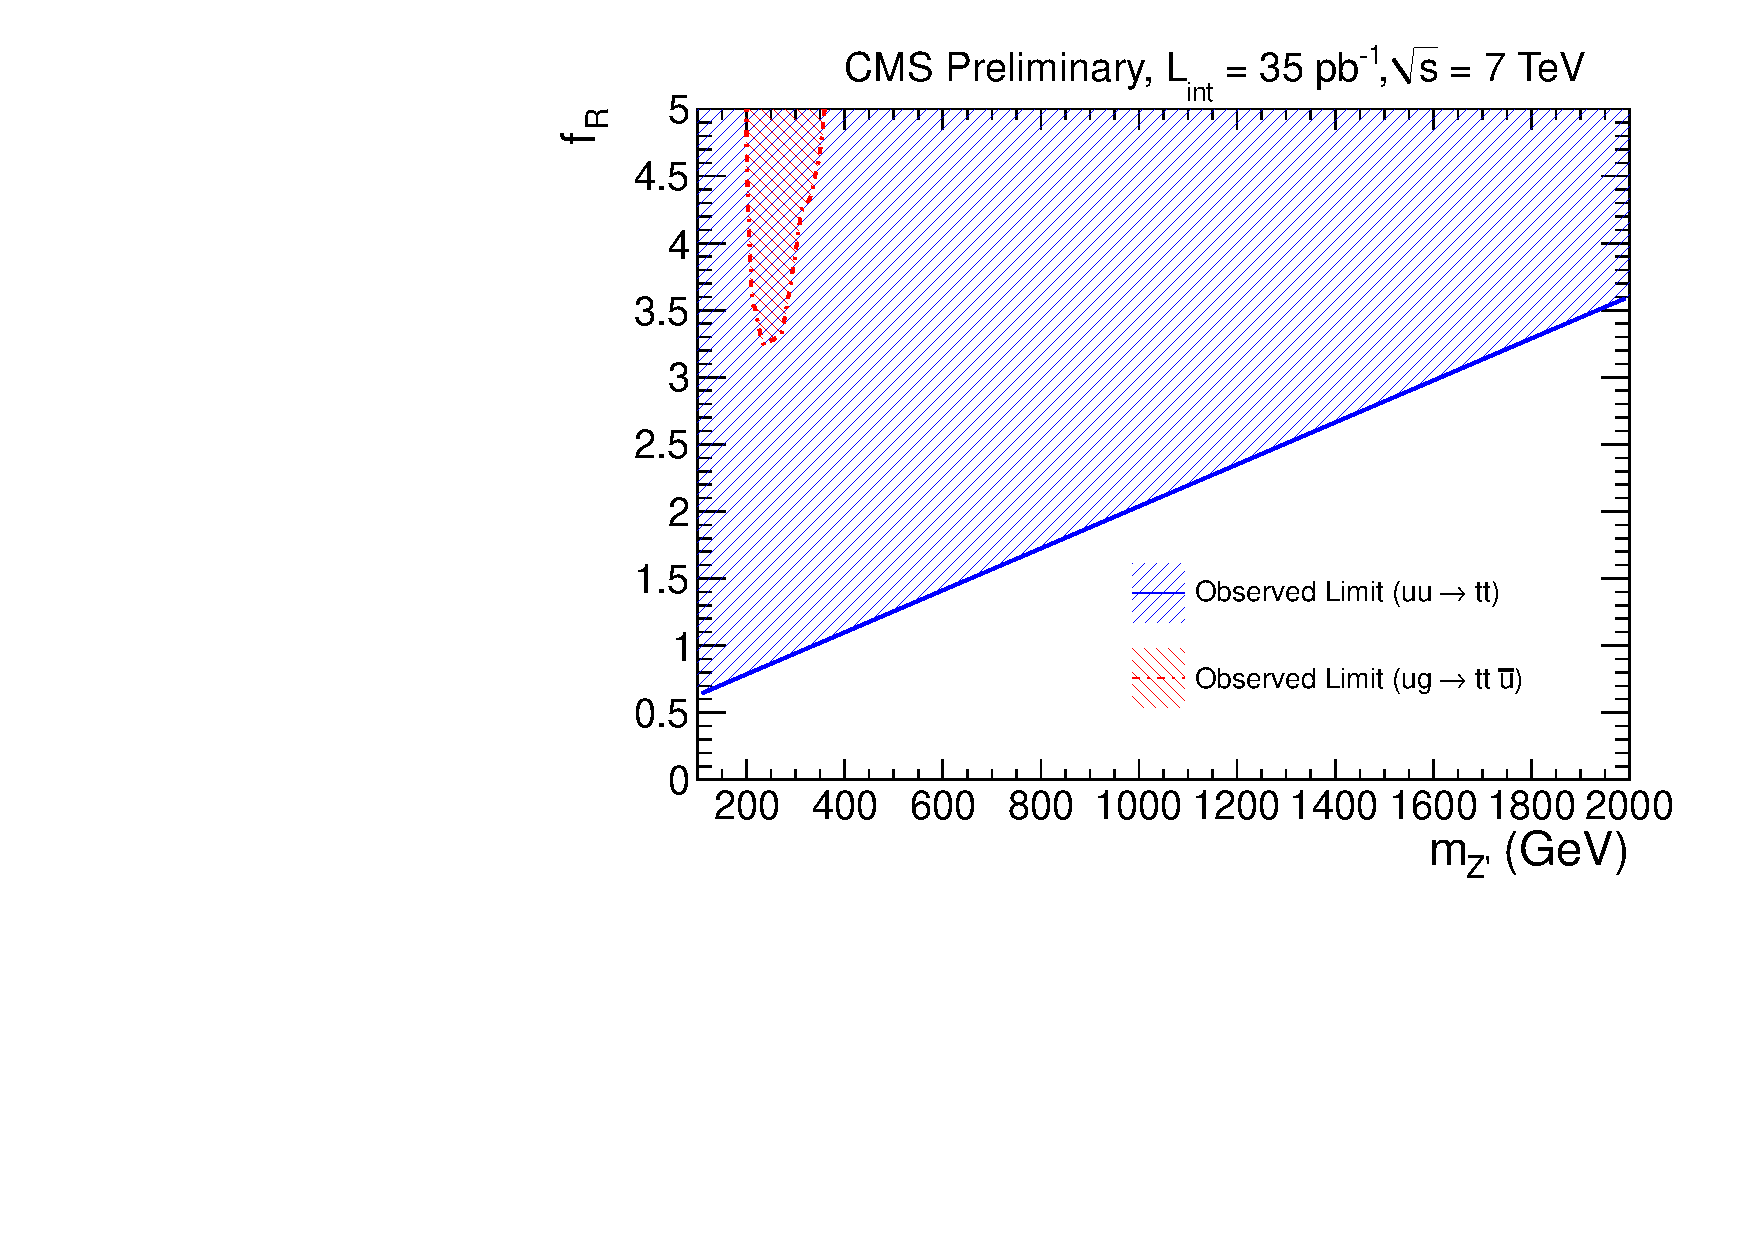
\includegraphics[width=0.7\linewidth]{figs/sstop_result.pdf}
\caption{ The exclusion region at 95\% CL. as a function of $Z'$ mass for various choices of the 
right-handed coupling, $f_R$. The solid lines represents regions due to t-channel exchange, where
as the dotted line excludes the assumptions on $ttj$ pair production. For the renormalization and factorization 
scales, $\mu$ is set to the top mass. \label{fig:sstopexclusion}}
\end{center}
\end{figure}

\begin{figure}[htb]
\begin{center}
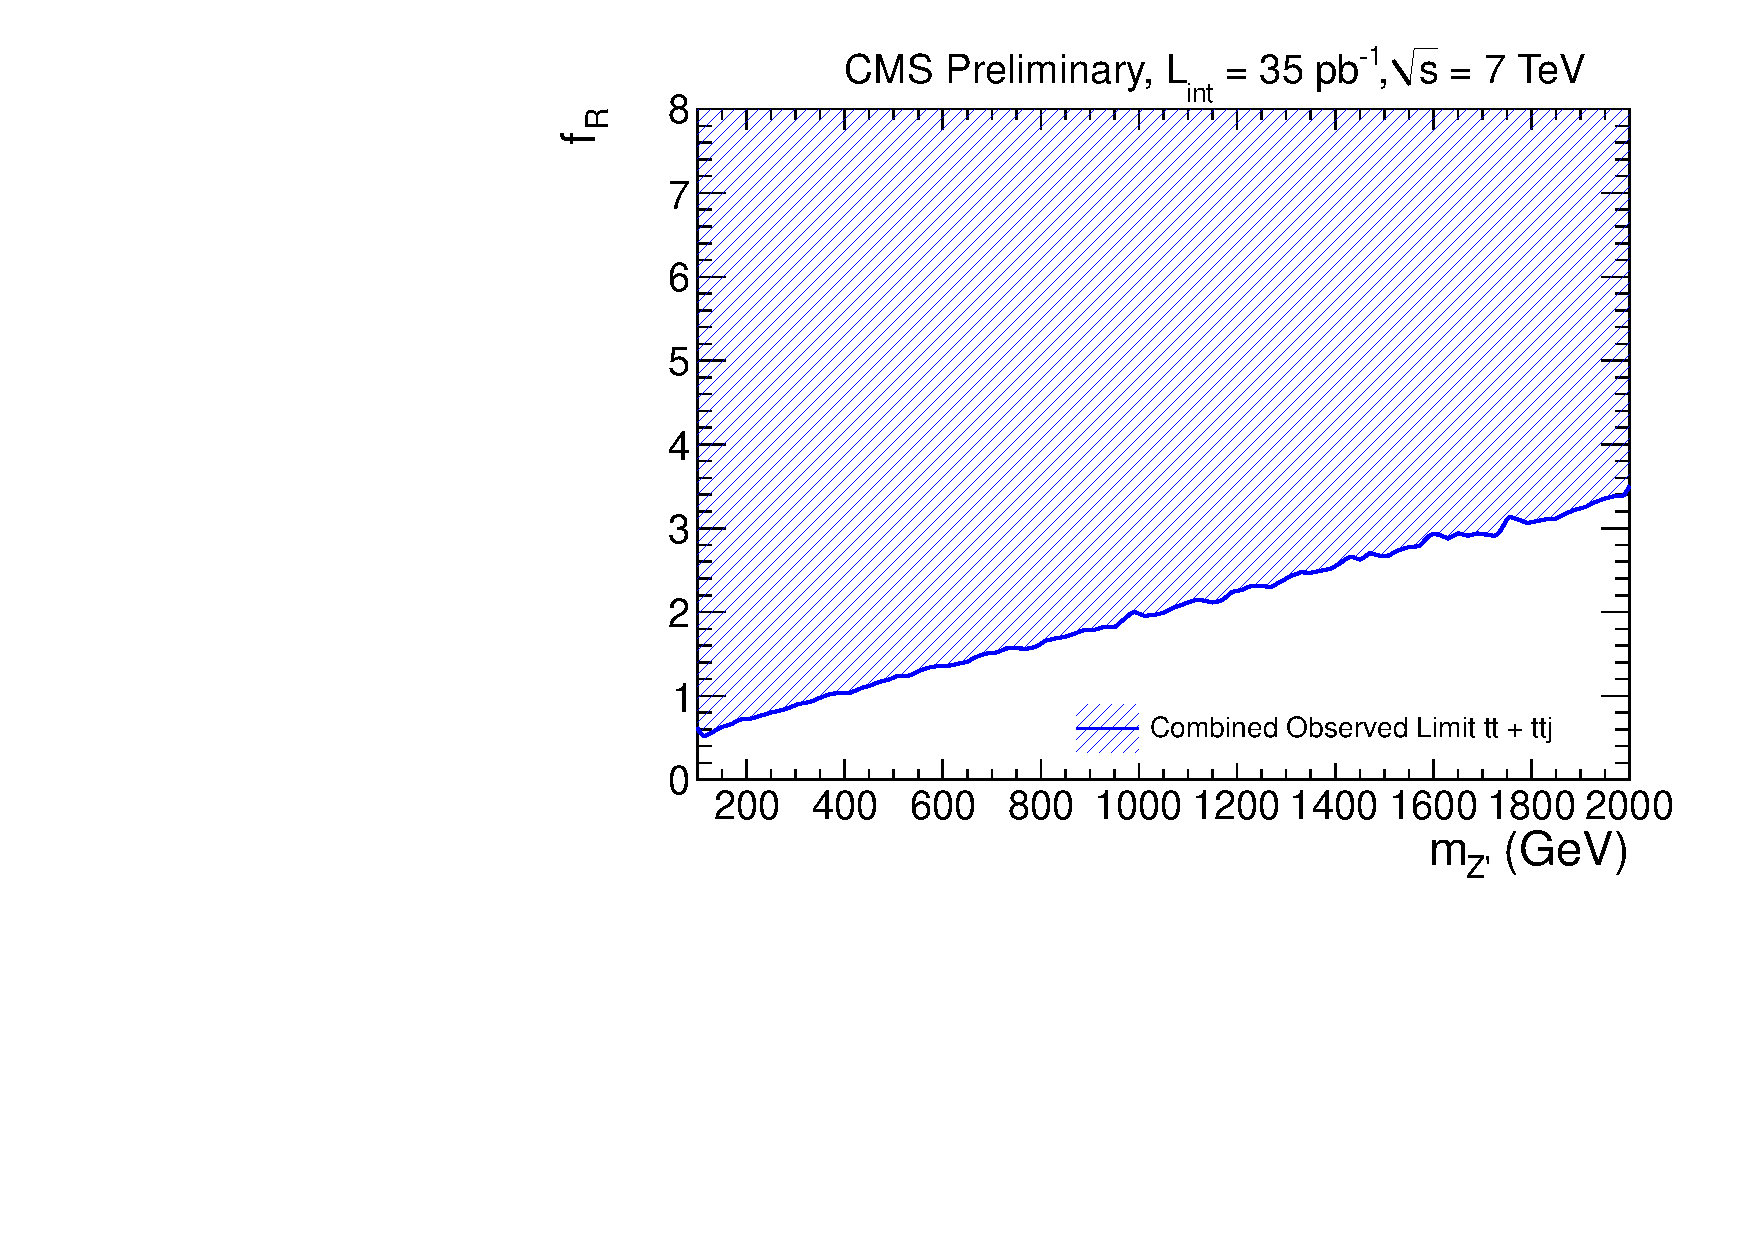
\includegraphics[width=0.7\linewidth]{figs/sscomb.pdf}
\caption{ The combined exclusion region at 95\% CL. as a function of $Z'$ mass for various choices of the 
right-handed coupling, $f_R$. Both t- and s-channel diagrams are added to get the combined exclusion limit
on same sign top production at the LHC. For the renormalization and factorization 
scales, $\mu$ is set to the top mass. \label{fig:sstopcombexclusion}}
\end{center}
\end{figure}

\section{Opposite Sign Dileptons}
\label{sec:osstudies}

This section summarizes the results of the SUSY parameter space scan
in the opposite sign dilepton channel. The measurement technique is
described in detail in a CMS note~\cite{osnote}. The technique
utilizes a data-driven method to estimate background characterized
by the presence of two high $P_T$, isolated, opposite sign leptons,
large $\met$, and significant jet activity. This generic signature is
sensitive to many new physics scenarios such as SUSY.  For the purposes
of this note we restrict ourselves to the $ee$, $e\mu$, and $\mu\mu$
final states, {\em i.e.}, we do not consider $\tau$'s, except in the
case that the $\tau$ decays leptonically. 

As we will show in Section~\ref{sec:osyields}, for a reasonable event
selection the main background is \ttbar decays. The data-driven
background prediction is based on a suggestion by Victor
Pavlunin~\cite{victor}. The idea is that in dilepton \ttbar events
the leptons and neutrinos from $W$ decays have on average the same
$P_T$ spectrum (modulo effects of $V-A$). One can then use the {\bf
observed} \ptll $~\equiv~|\vec{P}_T(\ell_1) + \vec{P}_T(\ell_2)|$
distribution to model the sum of neutrino $P_T$'s which is identified
with $\met$. 

\subsection{Event Yields}
\label{sec:osyields}

The expected event yields in 100~pb$^{-1}$ after applying the event selections
described in Section~\ref{sec:eventselection} to the data sets described in
Section~\ref{sec:datasamples} are detailed below: the SM yields are listed in
Table~\ref{tab:osyields}, and the mSUGRA scan point yields are illustrated in
Fig.~\ref{fig:hobs175_100pb}.

In Fig.~\ref{fig:smvictory} one sees the SM $\met$ distribution predicted
by the data-driven background estimation technique compared with the actual 
SM $\met$ distribution. The predicted $\met$ distribution
is the $\ptll$ distribution scaled to account for the $\met>$50 GeV cut; the scale
factor is about 1.6. The predicted event yield for a given $\met$ cut is then obtained by integrating
over the $\ptll$ distribution starting from the corresponding $\ptll$ value. 
For $\met>$175 GeV, the method predicts
3.9$\pm$0.51 SM events. The true yield is 4.3$\pm$0.27 SM events, which agrees
well with the prediction. The reported errors are statistical only.

\begin{table}[hbt]
\begin{center}
\begin{tabular}{|l|c|c|c|c|}\hline
Sample           & tcMET $>$ 175   \\ \hline
$t\overline{t}$  &   3.99          \\ 
$WW$             &   0.19          \\ 
$WZ$             &   0.01          \\ 
$ZZ$             &   0.01          \\ 
$W$+jets         &   0             \\
$Z$+jets         &   0             \\ 
Single top       &   0.05          \\ \hline
\end{tabular}
\caption{Expected SM event yields in 100~pb$^{-1}$.\label{tab:osyields}}
\end{center}
\end{table}

\begin{figure}[htb]
\begin{center}
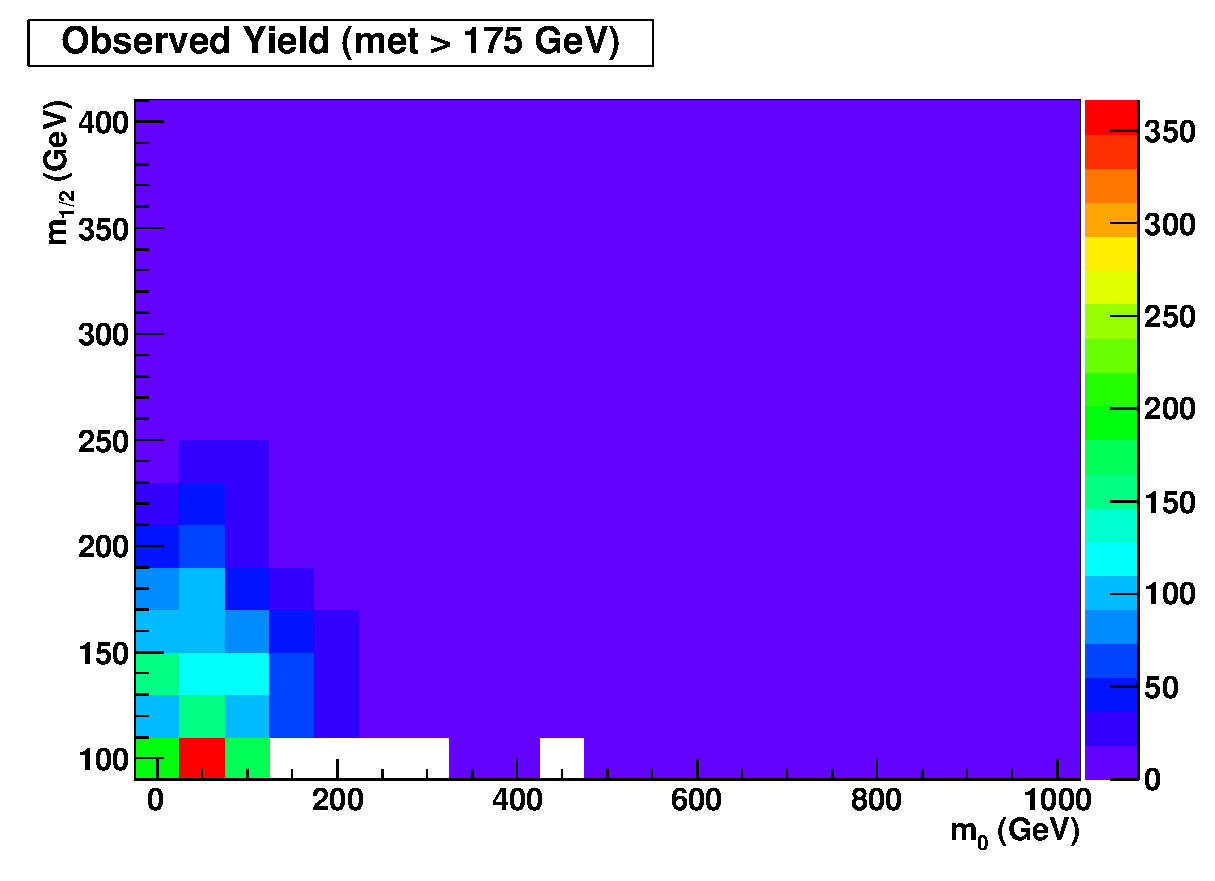
\includegraphics[width=0.7\linewidth]{figs/hobs175_100pb.eps}
\caption{Expected mSUGRA scan point event yields in 100~pb$^{-1}$\label{fig:hobs175_100pb}}
\end{center}
\end{figure}

\begin{figure}[htb]
\begin{center}
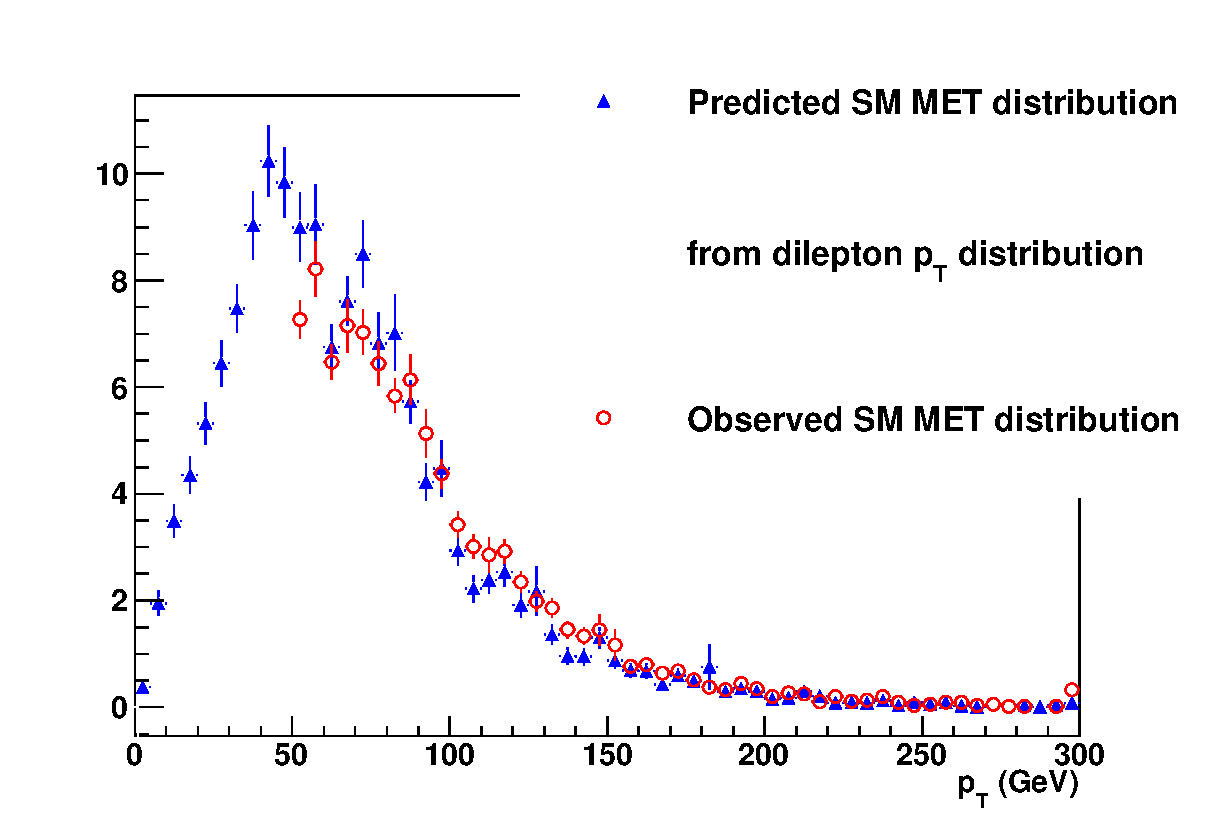
\includegraphics[width=0.7\linewidth]{figs/smvictory.eps}
\caption{Rescaled $\ptll$ distribution in the SM cocktail used to predict the $\met$ in blue, compared with the $\met$ in red.\label{fig:smvictory}}
\end{center}
\end{figure}


\subsection{Procedure for Determining $5\sigma$ Discovery Reach}
\label{sec:significance}

We  determine the  $5\sigma$  discovery reach  in the  $m_{0}-m_{1/2}$
plane by  performing our analysis at  each of the  mSUGRA scan points.
For each  point, we  determine the distributions  of $p_{T}(\ell\ell)$
and $\met$ and add these  to the corresponding SM distributions.  Then
we  perform   the  data-driven   background  estimate  by   using  the
$p_{T}(\ell\ell)$ to predict the  number of events with $\met>175$~GeV
(predicted background yield), as well  as directly count the number of
events which pass  this $\met$ cut (observed yield).   We quantify the
significance  of  the  discrepancy  between  the  observed  yield  and
predicted   background  yield   using  two   significance  estimators:
$Z_{Bi}$~\cite{cite:cousins}    and    $Z_N$~\cite{cite:conway}.   The
quantities required to calculate these estimators are:

\begin{itemize}
\item The predicted background yield
\item The relative systematic  uncertainty on the predicted background
yield (set to 25\%)
\item The  statistical uncertainty  on the predicted  background yield
($Z_N$ only, set to 0)
\item The observed yield
\end{itemize}

In   Figs.~\ref{fig:zbi} and~\ref{fig:zn} we   display  the
$Z_{Bi}$ and $Z_{N}$  significances, respectively,  assuming    integrated    luminosities   of
$100~\mathrm{pb}^{-1}$  and  $1~\mathrm{fb}^{-1}$.

\begin{figure*}[t]
\begin{center}
\begin{tabular}{c c}
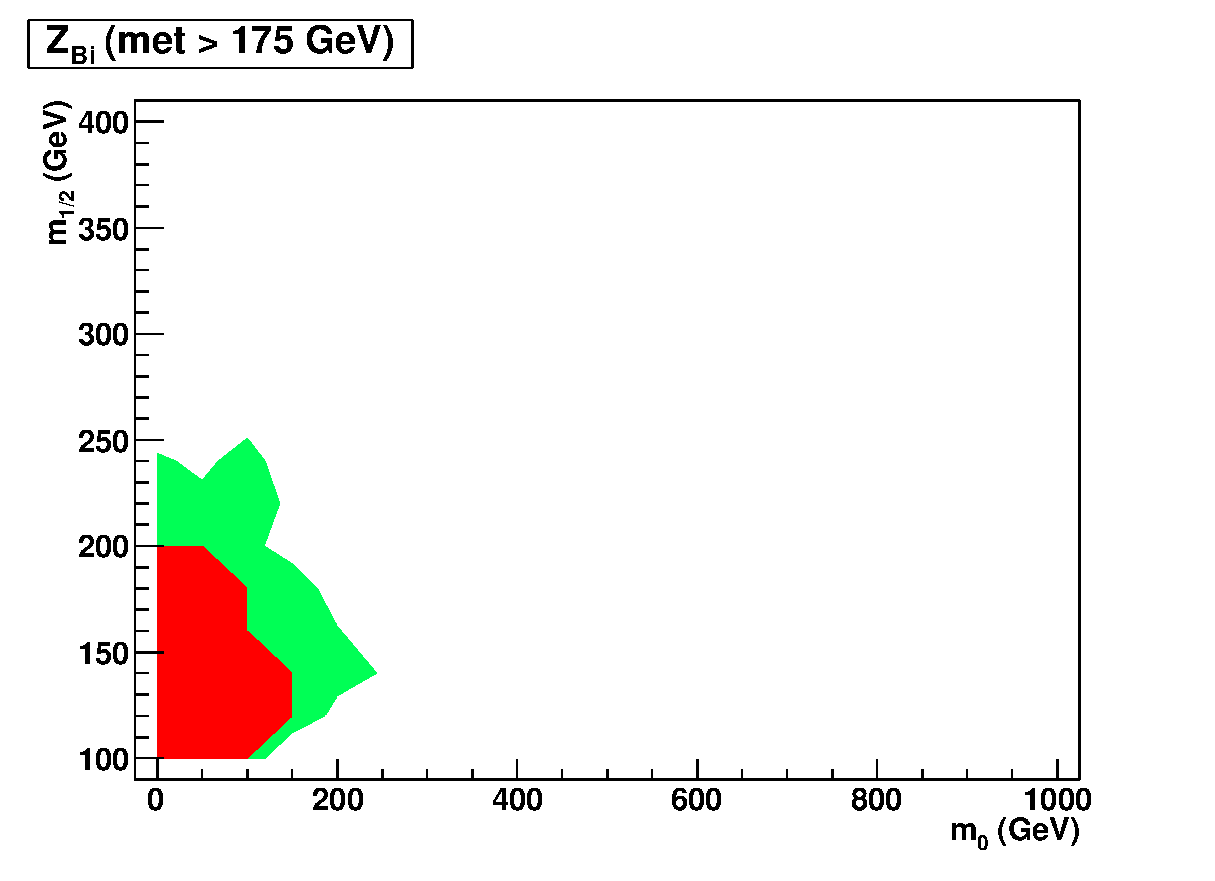
\includegraphics[height=5.5cm,clip=]{figs/hzbi175_100pb.eps}           &
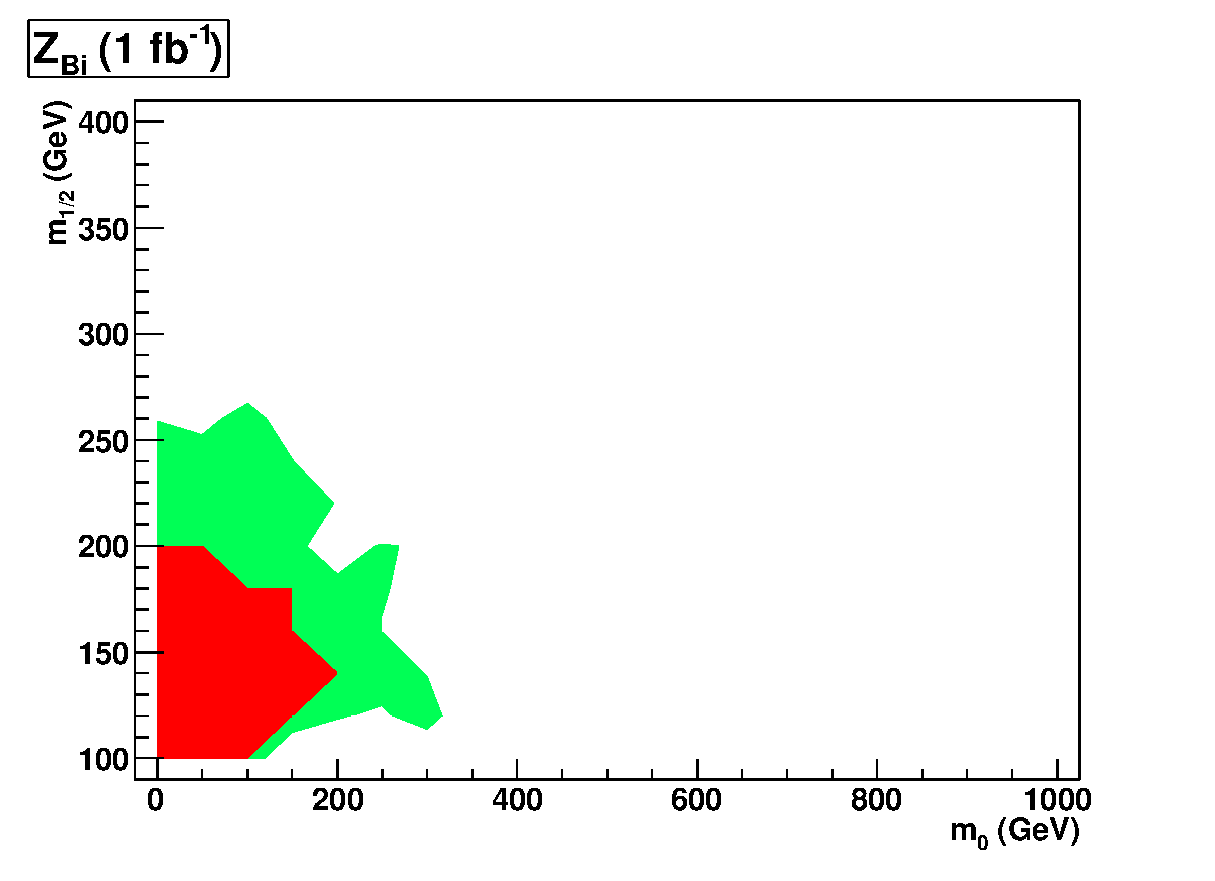
\includegraphics[height=5.5cm,clip=]{figs/hzbi175_1fb.eps}
\end{tabular}
\end{center}
\caption{The  $Z_{Bi}$  significance   in  the  $m_{0}-m_{1/2}$  plane
assuming  an  integrated  luminosity of  $100~\mathrm{pb}^{-1}$ (left)
and $1~\mathrm{fb}^{-1}$ (red). The red (green) shaded region indicates the
5$\sigma$ (3$\sigma$) sensitivity reach.   \label{fig:zbi}}
\end{figure*}

\begin{figure*}[b]
\begin{center}
\begin{tabular}{c c}
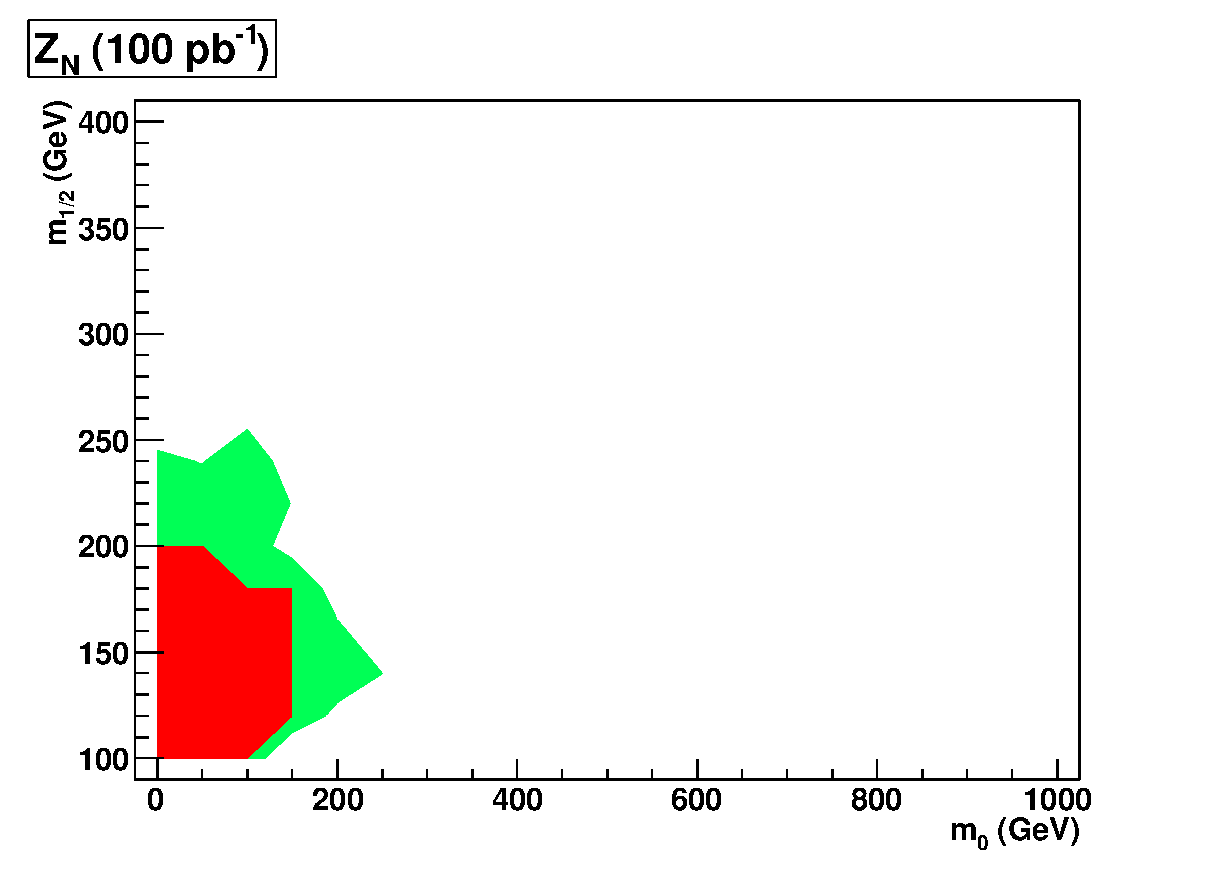
\includegraphics[height=5.5cm,clip=]{figs/hzn175_100pb.eps}           &
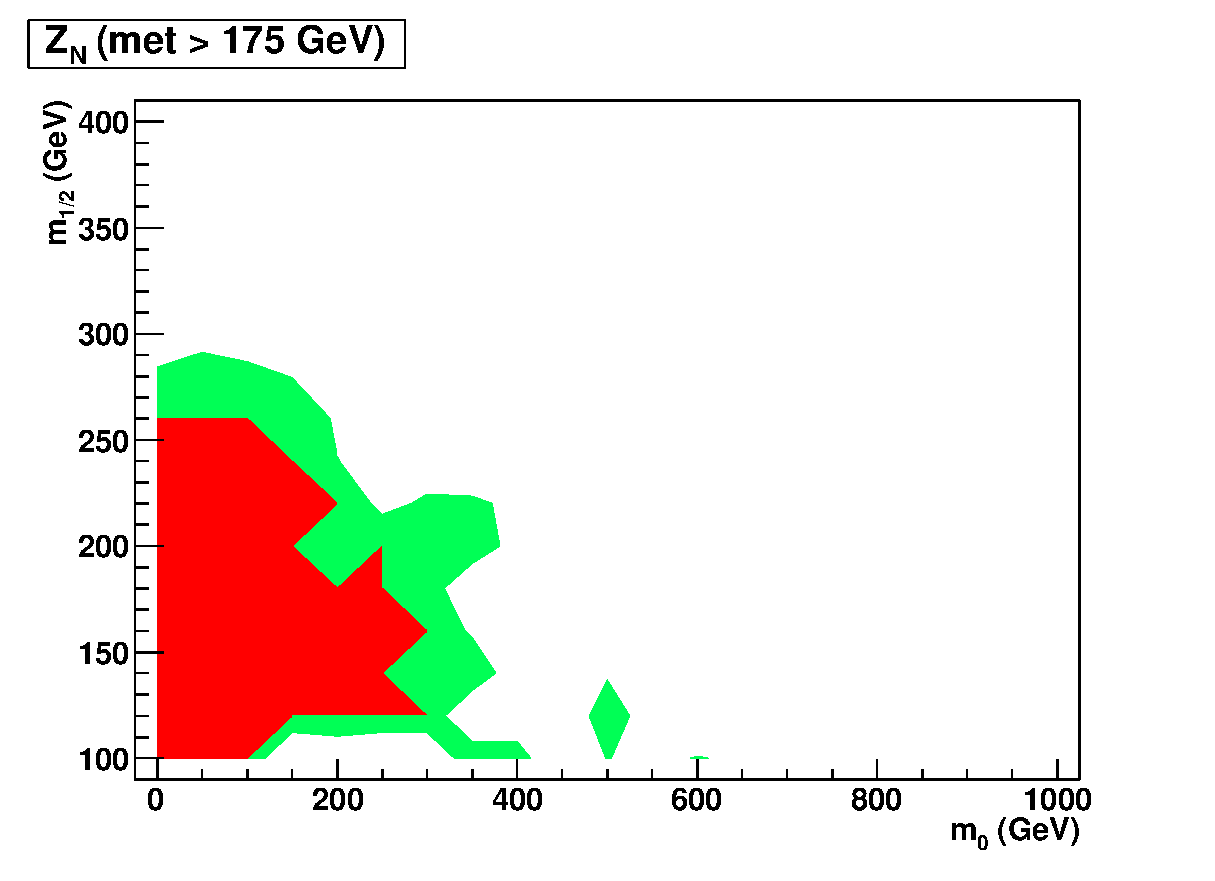
\includegraphics[height=5.5cm,clip=]{figs/hzn175_1fb.eps}
\end{tabular}
\end{center}
\caption{The  $Z_{N}$  significance   in  the  $m_{0}-m_{1/2}$  plane
assuming  an  integrated  luminosity of  $100~\mathrm{pb}^{-1}$ (left)
and $1~\mathrm{fb}^{-1}$ (red). The red (green) shaded region indicates the
5$\sigma$ (3$\sigma$) sensitivity reach.   \label{fig:zn}}
\end{figure*}


\subsection{Procedure for Excluding a Region of the mSUGRA Parameter Space}
\label{sec:exclusion}

Next we  determine the region of  the mSUGRA parameter  space which we
expect  to exclude  at 95\%  confidence level  (CL) if  we do  not see
evidence  for  signal  in data.   We  assume  that  we find  the  same
predicted background yield  and observed yield in data  that we expect
to  find based on  our SM  MC. We  use this  information to  exclude a
subset of the mSUGRA points using the following procedure.

The first  step is to  determine the 95\%  CL upper limit (UL)  on the
signal yield using a Bayesian  method from John Conway, implemented in
the program bayes.f. The required  inputs are: the observed yield, the
relative  uncertainty in  the  signal acceptance  (set  to 15\%),  the
predicted  background yield,  and  the total  error  on the  predicted
background yield. We evaluate this  error as the quadrature sum of the
systematic error (set  to 25\% of the predicted  background yield) and
the  statistical   uncertainty,  equal  to   $k\sqrt{N_{BKG}}$,  where
$k\approx1.6$ is  the scaling factor applied  to the $p_{T}(\ell\ell)$
distribution to  account for the  $\met>50~$GeV cut, and  $N_{BKG}$ is
the   predicted    background   yield.    We   find    an   error   of
$\sigma_{BKG}=3.4$     for     100~pb$^{-1}$     ($N_{BKG}=4$)     and
$\sigma_{BKG}=14.2$ for 1~fb$^{-1}$  ($N_{BKG}=40$). These values lead
to  95\% CL  ULs  of 7.6  signal  events and  33.1  signal events  for
100~pb$^{-1}$ and  1~fb$^{-1}$, respectively. It should  be noted that
bayes.f assumes a Gaussian  error distribution, while for our analysis
(especially  at 100~pb$^{-1}$ where  the background  yield is  4), our
errors are Poisson-distributed.

Next, we  wish to exclude mSUGRA  points based on the  signal yield UL
derived above.   The most obvious  way to do  so is to  exclude points
which  lead  to a  difference  between  observed  yield and  predicted
background yield  which exceeds the  UL on the signal  yield. However,
due to the effects of  signal contamination, which in our analysis can
lead to large biases in  the background prediction, one cannot rely on
this difference for exclusion. Consider an mSUGRA point which leads to
an observed yield  of 110 and a predicted background  yield of 100 for
an  integrated luminosity  of 100~pb$^{-1}$.   Since  $110-100>7.6$ we
would exclude  this point using  as our metric the  difference between
observed  and predicted  yields. However,  the  statistical difference
between these yields  is only at the $\approx1\sigma$  level and hence
this point should  not be excluded at 95\% CL. Instead,  we use as our
metric  the {\em  significance}  of the  discrepancy between  observed
yield and predicted background  yield, quantified by $Z_{Bi}$.  First,
we determine the $Z_{Bi}$ significance  corresponding to the UL on the
total yield ({\em  ie.}  the observed yield plus the  UL on the signal
yield) compared  to the predicted  background yield, again  assuming a
relative systematic  uncertainty of  25\% on the  predicted background
yield.  For  100~pb$^{-1}$ we find $Z_{Bi}=2.5$ for  an observed yield
of 4+7.6=11.6 and predicted background  of 4, while for 1~fb$^{-1}$ we
find $Z_{Bi}=2.2$ for an  observed yield of 40+33.1=73.1 and predicted
background of 40.  Finally, we  exclude those mSUGRA points which lead
to  a larger  $Z_{Bi}$  significance between  the  observed yield  and
predicted   background  yield   than   these  values,   as  shown   in
Fig.~\ref{fig:exc}   for 100~pb$^{-1}$  and
1~fb$^{-1}$.


\begin{figure*}[b]
\begin{center}
\begin{tabular}{c c}
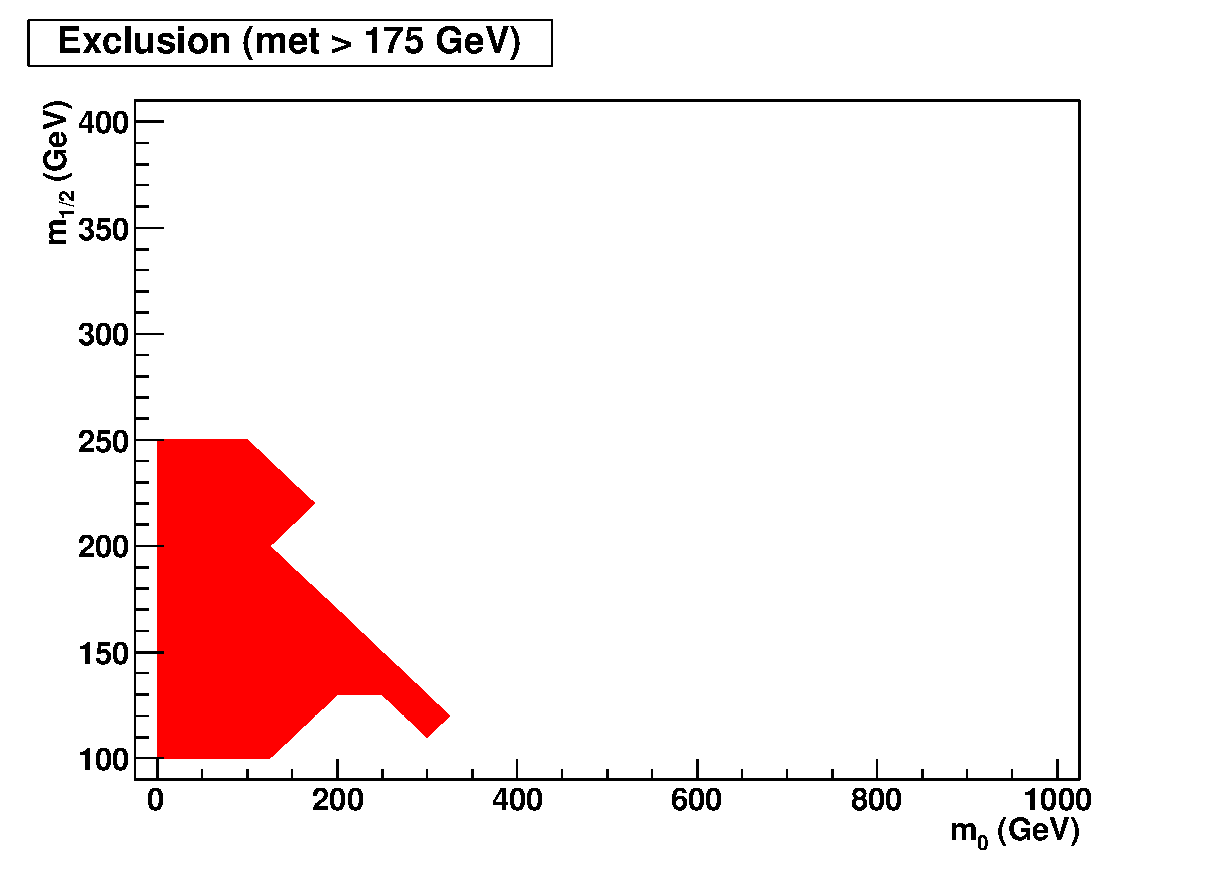
\includegraphics[height=5.5cm,clip=]{figs/hexc175_100pb.eps}           &
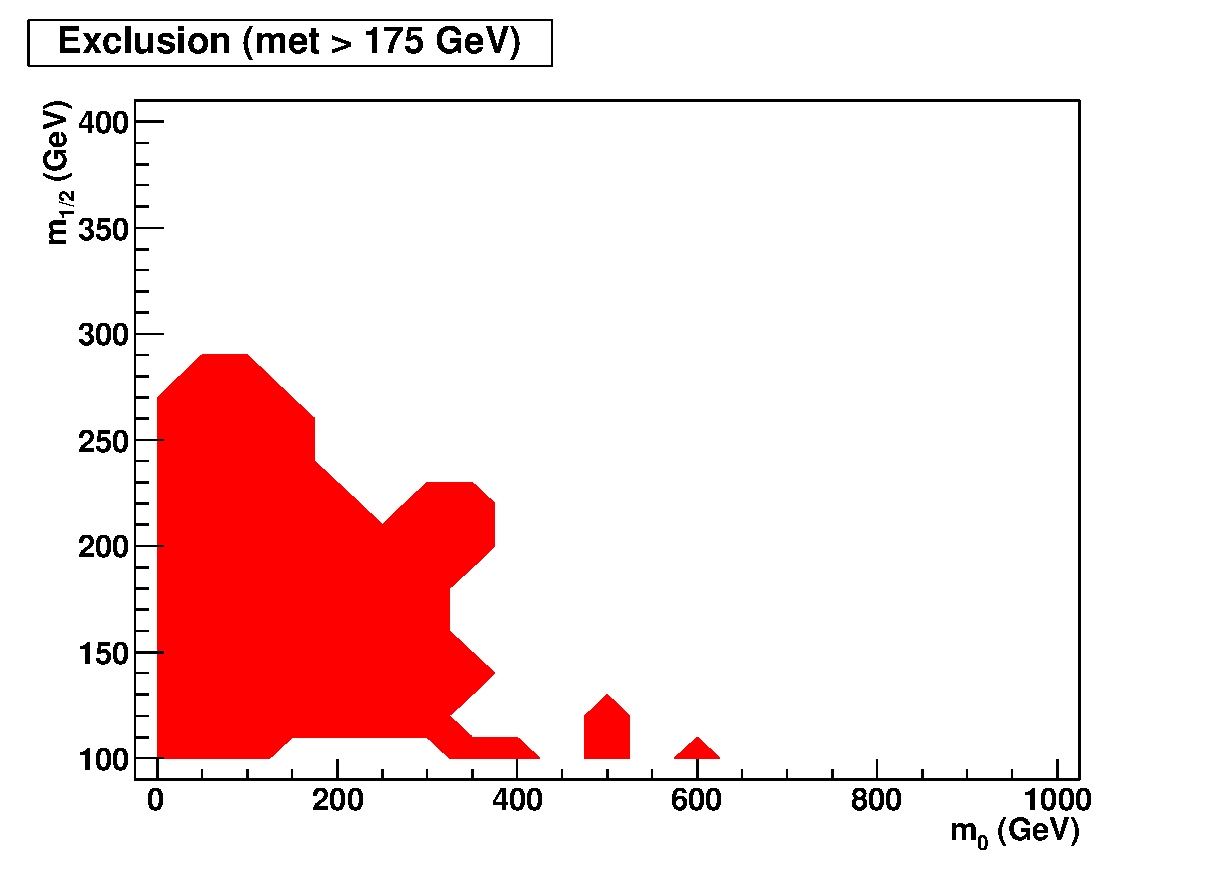
\includegraphics[height=5.5cm,clip=]{figs/hexc175_1fb.eps}
\end{tabular}
\end{center}
\caption{The excluded region (red  shaded area) of the $m_{0}-m_{1/2}$
plane       assuming      an       integrated       luminosity      of
$100~\mathrm{pb}^{-1}$ (left) and $1~\mathrm{fb}^{-1}$ (right). 
\label{fig:exc}}
\end{figure*}


\section{Conclusion}
\label{sec:conclusion}

We have assessed the sensitivity to mSUGRA of a generic signal characterized by two isolated, high $p_T$ leptons,
significant jet activity, and \met. We performed a scan of the mSUGRA $m_{0}-m_{1/2}$ parameter space and determined  
the expected excluded region in the case of no observed signal as well as the $5\sigma$ sensitivity reach for both SS
and OS dileptons, assuming integrated luminosities of 100 pb$^{-1}$ and 1 fb$^{-1}$. Our results indicate that we are sensitive to a
significant region of the mSUGRA parameter space which extends upon previous results from the Tevatron. 



\clearpage
\begin{thebibliography}{99}

\bibitem{cdf:recentSusy} {CDF Trilepton Search, 2009, CDF/PUB/EXOTIC/PUBLIC/9817};\\
{\small \tt http://www-cdf.fnal.gov/physics/exotic/r2a/20090521.trilepton\_3fb/Welcome.html}
%\bibitem{cdf:recentSusy1} {``Inclusive Search for Squark and Gluino Production in $p\bar{p}$ Collisions at $\sqrt{s}$ = 1.96-TeV'', Phys.Rev.Lett.102:121801, (2009).}
\bibitem{d0:recentSusy} {``Search for associated production of charginos and neutralinos in the trilepton final state using 2.3 fb$^{-1}$ of data'', Phys. Lett. B 680, 34 (2009).}
%\bibitem{d0:recentSusy1} {``Search for squarks and gluinos in events with jets and missing transverse energy using 2.1 fb$^{-1}$ of ppbar collision data at $sqrt(s)=1.96$ TeV'', 
%Phys. Lett. B 660 , 449 (2008).}

\bibitem{osnote} {``Data driven background estimate for a new physics search with opposite sign dileptons''}, CMS AN-2009/130.

\bibitem{ssnote} {``Data driven background study for new physics searches with same sign dileptons at $\sqrt{s} = 10 $ TeV''}, CMS AN-2009/138.

\bibitem{mcsusy}{\tt https://twiki.cern.ch/twiki/bin/viewauth/CMS/SUSYMCRequirements0911}.

\bibitem{fast10}{\tt https://twiki.cern.ch/twiki/bin/view/CMS/SUSY33XScan}.

\bibitem{ww} {``Prospects for measuring the $WW$ production cross section in $pp$ collisions at $\sqrt s = $10 TeV''}, CMS AN-2009/042 and PAS EWK-09-002.

\bibitem{ttbar} {``Expectations for observation of top quark pair production in the dilepton final state with the early CMS data''}, CMS AN-2009/050 and PAS TOP-09-002.

\bibitem{tcmet} {``Correcting Missing Transverse Energy Using Tracks``} CMS AN-2009/022.

\bibitem{conversionnote} {``Study of photon conversion rejection at CMS''}, CMS AN-2009/159.

\bibitem{glbtrk} {\tt https://hypernews.cern.ch/HyperNews/CMS/get/muon/258.html}.

\bibitem{muonid} {``Muon Identification in CMS''}, CMS AN-2008/098.

\bibitem{vplusj} {\tt https://twiki.cern.ch/twiki/bin/view/CMS/VplusJets}.

\bibitem{fakenote} {``Data-driven methods to estimate the electron and muon fake contributions to lepton analyses''}, CMS AN-2009/041.

\bibitem{cite:cousins} {``Evaluation of three methods for calculating statistical significance when incorporating a systematic uncertainty into a test of the background-only hypothesis for a Poisson process''} arXiv:physics/0702156 [physics.data-an]

\bibitem{cite:conway} {``Interval estimation in the presence of nuisance parameters. 1. Bayesian approach''} arXiv:physics/0409129v1 [physics.data-an]

\bibitem{lep:lepsusyreach}{LEP Susy working group: {\tt http://lepsusy.web.cern.ch/lepsusy/} }

\bibitem{bayes}{\tt http://arxiv.org/pdf/physics/0409129}

\bibitem{victor} {\tt http://arxiv.org/pdf/0906.5016}; \\
{\tt http://indico.cern.ch/contributionDisplay.py?contribId=2\&confId=39042}.

\bibitem{summer09}{\tt https://twiki.cern.ch/twiki/bin/view/CMS/SUSY31XProduction}.


\end{thebibliography}

\clearpage
%\section{appendix}
\label{sec:tables}




\vspace{30 mm}
\begin{figure}[htb]
\begin{center}
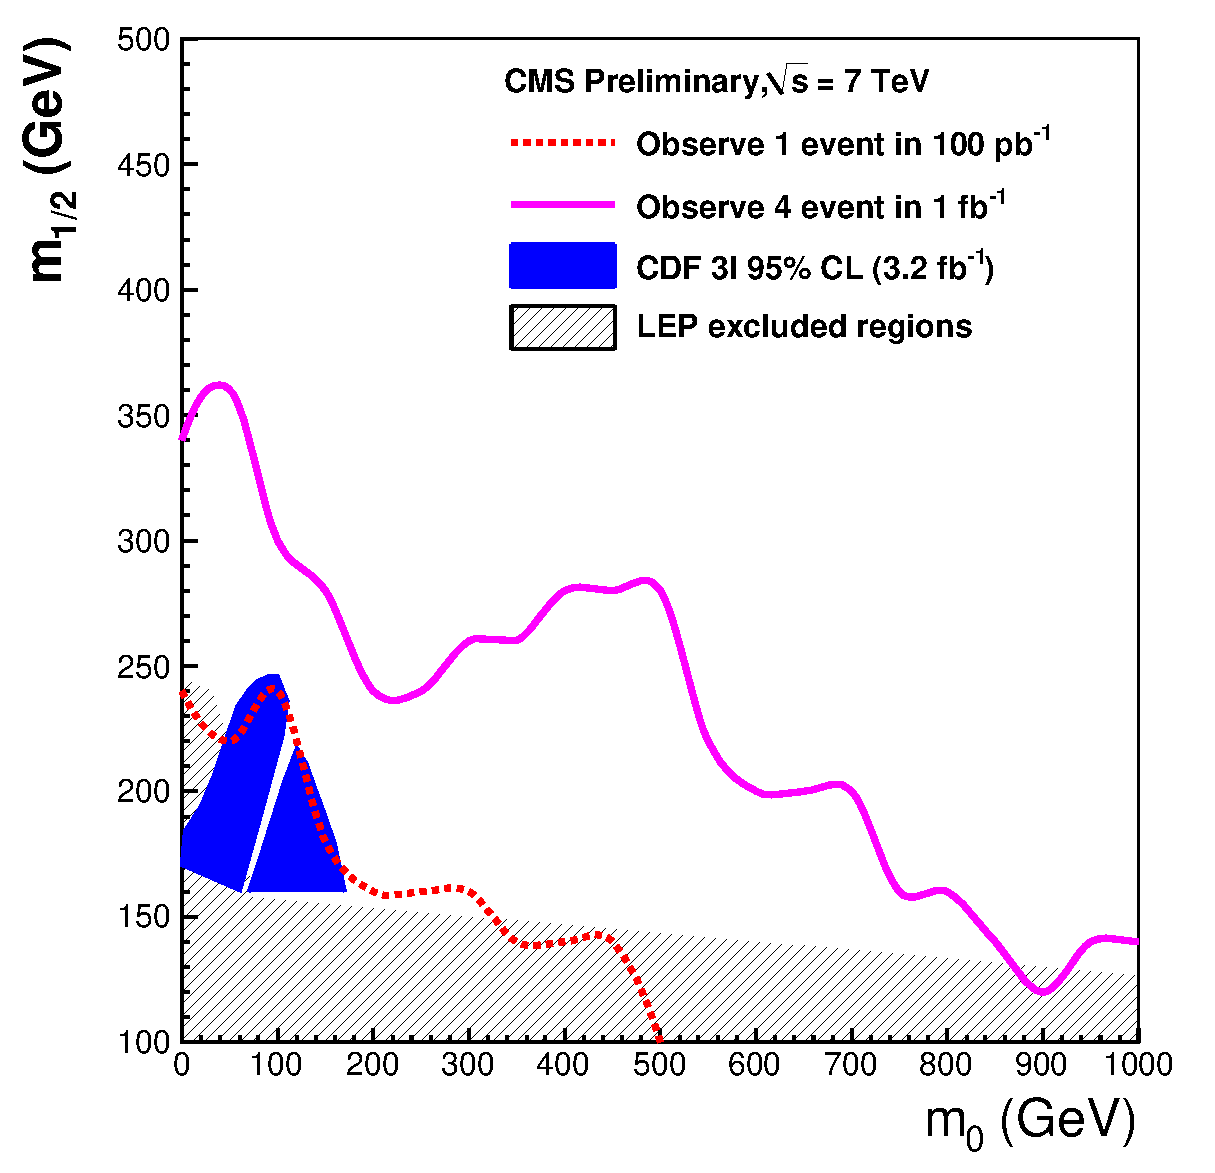
\includegraphics[width=0.7\linewidth]{figs/exclusion1fbssa.eps}
\caption{The $m_{0}-m_{1/2}$ exclusion plot at the 95\% CL in the framework of
mSUGRA assuming R-parity conservation using an  integrated  luminosity of
$100~\mathrm{pb}^{-1}$ and $1~\mathrm{fb}^{-1}$. The blue region
was excluded by the CDF experiment~\cite{cdf:recentSusy}. The black hashed region was excluded by the LEP experiments~\cite{lep:lepsusyreach}.
\label{fig:ssadd_exclusion}}

\end{center}
\end{figure}


\begin{table}[hbt]
\begin{center}
\renewcommand{\arraystretch}{2.0}
 {\footnotesize
\begin{tabular}{|l|c|c|c|c|c|c|c|c|}\hline
$m_{0}$ GeV & $m_{1/2}$ GeV & Event Yield & Raw Event Yield \\ \hline
0 & 240.0 & 5.2 $\pm$ 0.6 & 84.0 $\pm$ 9.2 \\ 
50 & 240.0 & 3.3 $\pm$ 0.4 & 56.0 $\pm$ 7.5 \\ 
100 & 260.0 & 4.7 $\pm$ 0.4 & 130.0 $\pm$ 11.4 \\ 
150 & 260.0 & 4.6 $\pm$ 0.4 & 139.0 $\pm$ 11.8 \\ 
200 & 200.0 & 3.6 $\pm$ 0.7 & 30.0 $\pm$ 5.5 \\ 
250 & 180.0 & 4.1 $\pm$ 0.8 & 24.0 $\pm$ 4.9 \\ 
300 & 180.0 & 4.6 $\pm$ 0.8 & 32.0 $\pm$ 5.7 \\ 
350 & 200.0 & 3.4 $\pm$ 0.5 & 45.0 $\pm$ 6.7 \\ 
400 & 140.0 & 10.3 $\pm$ 1.8 & 31.0 $\pm$ 5.6 \\ \hline
\end{tabular} }
\caption{Expected weighted and raw event yields in mSUGRA $m_{0}-m_{1/2}$ plane with tan$\beta = 3$, A$_0 = 0$, $\mu > 0$. The weighted yields are normalized to 100 pb$^{-1}$ of integrated luminosity and are used in case of 0 observed event hypothesis. Uncertainties are from MC statistics. \label{tab:ssyields_ex0}}
\end{center}
\end{table}

\vspace{10 mm}
\begin{table}[hbt]
\begin{center}
\renewcommand{\arraystretch}{2.0}
 {\footnotesize
\begin{tabular}{|l|c|c|c|c|c|c|c|c|}\hline
$m_{0}$ GeV & $m_{1/2}$ GeV & Event Yield & Raw Event Yield \\ \hline
0 & 240.0 & 5.2 $\pm$ 0.6 & 84.0 $\pm$ 9.2 \\ 
50 & 220.0 & 6.5 $\pm$ 0.8 & 68.0 $\pm$ 8.2 \\ 
100 & 240.0 & 6.6 $\pm$ 0.6 & 117.0 $\pm$ 10.8 \\ 
150 & 180.0 & 9.7 $\pm$ 1.5 & 42.0 $\pm$ 6.5 \\ 
200 & 160.0 & 10.3 $\pm$ 1.9 & 29.0 $\pm$ 5.4 \\ 
250 & 160.0 & 8.4 $\pm$ 1.6 & 28.0 $\pm$ 5.3 \\ 
300 & 160.0 & 6.5 $\pm$ 1.3 & 26.0 $\pm$ 5.1 \\ 
350 & 140.0 & 7.8 $\pm$ 1.8 & 20.0 $\pm$ 4.5 \\ 
400 & 140.0 & 10.3 $\pm$ 1.8 & 31.0 $\pm$ 5.6 \\ 
450 & 140.0 & 10.1 $\pm$ 1.7 & 36.0 $\pm$ 6.0 \\ 
500 & 100.0 & 6.8 $\pm$ 3.1 & 5.0 $\pm$ 2.2 \\ \hline
\end{tabular} }
\caption{Expected weighted and raw event yields in mSUGRA $m_{0}-m_{1/2}$ plane with tan$\beta = 3$, A$_0 = 0$, $\mu > 0$. The weighted yields are normalized to 100 pb$^{-1}$ of integrated luminosity and are used in case of 1 observed event hypothesis. Uncertainties are from MC statistics. \label{tab:ssyields_ex1}}
\end{center}
\end{table}

\vspace{10 mm}
\begin{table}[hbt]
\begin{center}
\renewcommand{\arraystretch}{2.0}
 {\footnotesize
\begin{tabular}{|l|c|c|c|c|c|c|c|c|}\hline
$m_{0}$ GeV & $m_{1/2}$ GeV & Event Yield & Raw Event Yield \\ \hline
0 & 340.0 & 10.9 $\pm$ 0.1 & 132.0 $\pm$ 11.5 \\ 
50 & 360.0 & 7.4 $\pm$ 0.1 & 130.0 $\pm$ 11.4 \\ 
100 & 300.0 & 10.4 $\pm$ 0.1 & 66.0 $\pm$ 8.1 \\ 
150 & 280.0 & 20.6 $\pm$ 0.2 & 95.0 $\pm$ 9.7 \\ 
200 & 240.0 & 14.3 $\pm$ 0.3 & 31.0 $\pm$ 5.6 \\ 
250 & 240.0 & 7.8 $\pm$ 0.2 & 19.0 $\pm$ 4.4 \\ 
300 & 260.0 & 7.6 $\pm$ 0.1 & 32.0 $\pm$ 5.7 \\ 
350 & 260.0 & 7.6 $\pm$ 0.1 & 36.0 $\pm$ 6.0 \\ 
400 & 280.0 & 8.8 $\pm$ 0.1 & 70.0 $\pm$ 8.4 \\ 
450 & 280.0 & 9.6 $\pm$ 0.1 & 86.0 $\pm$ 9.3 \\ 
500 & 280.0 & 8.0 $\pm$ 0.1 & 82.0 $\pm$ 9.1 \\ 
550 & 220.0 & 10.1 $\pm$ 0.2 & 36.0 $\pm$ 6.0 \\ 
600 & 200.0 & 10.8 $\pm$ 0.2 & 28.0 $\pm$ 5.3 \\ 
650 & 200.0 & 11.3 $\pm$ 0.2 & 32.0 $\pm$ 5.7 \\ 
700 & 200.0 & 10.0 $\pm$ 0.2 & 31.0 $\pm$ 5.6 \\ 
750 & 160.0 & 9.4 $\pm$ 0.3 & 11.0 $\pm$ 3.3 \\ 
800 & 160.0 & 8.0 $\pm$ 0.3 & 10.0 $\pm$ 3.2 \\ 
850 & 140.0 & 8.8 $\pm$ 0.4 & 6.0 $\pm$ 2.4 \\ 
900 & 120.0 & 12.2 $\pm$ 0.6 & 4.0 $\pm$ 2.0 \\ 
950 & 140.0 & 15.0 $\pm$ 0.5 & 11.0 $\pm$ 3.3 \\ 
1000 & 140.0 & 10.7 $\pm$ 0.4 & 8.0 $\pm$ 2.8 \\ \hline
\end{tabular} }
\caption{Expected weighted and raw event yields in mSUGRA $m_{0}-m_{1/2}$ plane with tan$\beta = 3$, A$_0 = 0$, $\mu > 0$. The weighted yields are normalized to 1 fb$^{-1}$ of integrated luminosity and are used in case of 4 observed event hypothesis. Uncertainties are from MC statistics. \label{tab:ssyields_ex1fb}}
\end{center}
\end{table}

\end{document}
